\documentclass[11pt,a4paper]{article}
\usepackage[pdftex]{graphicx}
\usepackage[utf8]{inputenc}
\usepackage[a4paper]{geometry}
\usepackage[hyphens]{url}

\makeatletter
\renewcommand\paragraph{\@startsection{paragraph}{4}{\z@}%
  {-3.25ex\@plus -1ex \@minus -.2ex}%
  {1.5ex \@plus .2ex}%
  {\normalfont\normalsize\bfseries}}
\makeatother
\setcounter{tocdepth}{3}
\begin{document}

\begin{titlepage}
\begin{center}

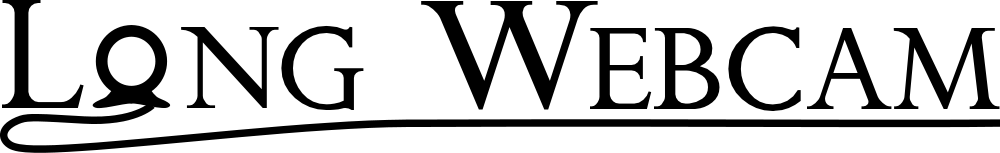
\includegraphics[width=0.85\textwidth]{./Logo_Large-cropped_black.png}

\vspace{3 cm}

\textbf{\Huge{Project Description}}

\vspace{1 cm}

\textit{\large{Version 2.0 - 16th September 2012}}

\vspace{4 cm}

\textbf{\Large{Authors:}}

\textbf{Steve Jones} (steve@longwebcam.org)

\end{center}

\end{titlepage}

\tableofcontents
\clearpage
\pagenumbering{roman}
\section*{Document History}
    \addcontentsline{toc}{section}{Document History}
\begin{table*}[tbhp!]
\begin{tabular}{ c c p{9.9cm} }
\textbf{Version} & \textbf{Date} & \textbf{Notes} \\
0.1 & 17 Nov 2011 & Document development; The version number will be held at 0.1 until all sections have been written. \\
1.0 & 26 Dec 2011 & First draft complete. \\
2.0 & 16 Sep 2012 & Extensive rewrite.
\end{tabular}
\end{table*}


\clearpage
\pagenumbering{arabic}
\section{Introduction}
This document outlines the background and goals of the Long Webcam project, which aims to produce time-lapse videos of landscapes over very long time periods. The document will serve as a high-level overview of all the features that the project will provide in some detail, but will not give any technical details of the manner in which those features will be implemented.

\subsection{Project Background}
The Long Webcam project has grown out of a fascination of all forms of time-lapse photography, together with an interest in the work of the Long Now Foundation (\url{http://www.longnow.org}). Time-lapse photography produces videos of events that take too long for conventional video to capture comfortably – single events that take hours or longer to complete. They allow us to see the changes in objects that our normal senses cannot easily comprehend – stars moving across the sky, flowers opening etc.
Some projects have recorded events of much longer time scales – construction of buildings, or the ageing of a person over several years. So far, though, there are no methods of capturing change on the scales at which landscapes changes. Trees grow and perish, glaciers advance and retreat, buildings are built and destroyed. Streets change around us. The Long Webcam project aims to capture such events over many years, and create an archive of our changing world.

\clearpage
\section{Using the Website}
The easiest way to describe the operation of the Long Webcam project is to describe the functions that will be available to users of the website. These functions will imply the data and features that the project will provide, which can then be described in more detail.

\subsection{Finding images}
The primary function of the Long Webcam site is to provide access to the images stored in its archive. Users will be able to use these images for a number of purposes. The fundamental purpose of the site is to allow users to locate images of interest.

\subsubsection{Cameras}
Since the whole purpose of this project is to look at changing scenes through time, it makes sense that the primary method of finding images of interest is to search for cameras; once a camera is located, the user will be able to look through the history of its images. Users are most likely to locate cameras in terms of the content of the captured images. Content of interest may be broadly categorised (e.g. cities, forests, landscapes etc.) or very specific (searching for specific locations or landmarks). The site will allow users to search for images in a number of ways to maximise the likelihood of locating the desired images.

\paragraph{Search by location}

It is likely that most users will search for cameras by their location. There are any number of ways to enter location information, and several of these will be provided by the site.

\subparagraph{User's location}

The latest web browsers allow sites to determine a user's current location (with the user's permission). If this information is not available, it is often possible to establish a user's approximate location using their IP address. The site will therefore be able to find cameras that are closest to the user.

\subparagraph{Browsing a map}

The site will allow users to navigate a map of the world to locate cameras. Google Maps is the most frequently seen implementation of this functionality. This could be extended to a Google Earth plugin in the future.

\subparagraph{Place name/address search}

Users will be allowed to enter place names or addresses (similar to the Google Maps search) to locate cameras near certain locations of interest. The level of detail that is available (countries, cities, postal codes etc.) will be dependent on the availability of geographical search information.

\subparagraph{Co-ordinates}

The user will be able to enter specific co-ordinates for searching by location. In the beginning this will be restricted to latitude/longitude, but may encompass other co-ordinate systems (e.g. Ordnance Survey grid references) in the future.

\paragraph{Search by category}

Each camera will be given a set of keywords describing its view. These keywords will be in the form of a category tree, so users can browse the categories for subjects that interest them.

\paragraph{Search by text}

Each camera will be given a title and a short piece of descriptive text to help users understand the focus of the images. This information will be fully searchable, allowing users to enter any words they wish to search for cameras.

\paragraph{Search by time coverage}

Some users will only be interested in finding cameras that have captured pictures during a specific period of time or a specific span of time.

\subsubsection{Events}
The Long Webcam project will record specific events of interest that are captured by its cameras. This may include natural disasters/events, construction or destruction of buildings, or any other happening that daily images capture in an interesting way. Users will be able to search for these events in order to obtain the images that show them.

\paragraph{Search by location}
As with cameras, users will be allowed to search for events near a specified location. All the location search options allowed for cameras will also be present for events.

\paragraph{Search by text}
As with cameras, each event will be given a name and have a short text description. This will allow free text search for events.

\paragraph{Search by event type}
Events will be given keywords from a category hierarchy similar to that for cameras. Users will therefore be able to find events matching those keywords.

\paragraph{Search by date}
Obviously, events will occur at specific times. Users will be allowed to locate events based on specified dates or ranges of dates.

\paragraph{Search by timeline}
The event search feature will allow users to view events in a timeline. This will give the function of browsing for items of interest through time.

\subsection{Using images}
The Long Webcam project exists to make its archive of images available to anybody. Users will be able to download any image they choose from the archve, or request a timelapse video to be generated from a camera for a specified time period.

\subsubsection{Licensing}
\label{section:licensing}
Use of images from the Long Webcam site will be subject to a licensing agreement to protect both the site's and camera owners' interests. The default agreement will be very broad allowing any non-commercial use without explicit permission but with credit to both the Long Webcam project and the camera owner. (The camera owner may wish to remain anoymous and uncredited. The project will allow the owner's name not to appear on the site, but their details will be kept by the project for contact and record-keeping purposes.) A Creative Commons licence is the most likely candidate for such a licence.

While all camera owners will be strongly encouraged to release their images under this generous licence, some may have very good reasons to have a more restrictive usage policy for their images. The Long Webcam project will respect these wishes and ensure that images are presented with the appropriate licensing terms. The site may also add watermarks to images and videos exported from the project if required.

\section{Cameras}
\label{cameras}
The webcams employed by the project will be maintained by individuals or organisations who will own the cameras together with any equipment required to maintain them and submit images to the Long Webcam site.

\subsection{Types of camera}
The Long Webcam site will support the collection of images from webcams in three different modes:

\begin{itemize}
\item Webcam publishing images to a web page
\item Webcam with software sending images to the Long Webcam site
\item Standalone webcam unit
    \begin{itemize}
    \item With network connection: sends images to the site automatically
    \item Without network connection: images must be manually uploaded to the site
    \end{itemize}
\end{itemize}

Where a webcam is already publishing captured images to a website, adding the daily image to the Long Webcam archive is trivial, and can be handled automatically by the Long Webcam server. Given a fixed URL for the webcam, it can simply download the image at midday (for the time zone in which the camera is located) and add it to the archive.

If a webcam is attached to a standard PC but does not upload captured images to a website, custom software can be written to run on the PC that captures a webcam image and uploads it to the Long Webcam site. As long as the PC is switched on and the software is running, no intervention will be required by the camera owner.

Standalone webcam units are intended for use where standard PC equipment is not appropriate. If they have a connection to the Internet, they will automatically take pictures and upload them to the Long Webcam site as a camera attached to a PC would. If no Internet connection is available, the units will take photos every day and store them on local media. The camera owner will be responsible for periodically collecting the pictures from the webcam unit and uploading them to the Long Webcam site. The design and operation of these standalone units is discussed in brief detail in Section~\ref{standalone}.

\subsubsection{Standalone webcam units}
\label{standalone}

The Long Webcam project will design standalone webcam units for the placement of cameras where standard equipment is not viable. The units will have various configuration options depending on the availability of mains electricity and Internet access. The fundamental components of the unit will consist of:

\begin{itemize}
\item Camera
\item Control board with software pre-loaded
\item Power supply:
\begin{itemize}
\item Mains power supply unit (if mains electricity is available)
\item Battery pack (if mains is not available)
\end{itemize}
\item Optional network access (wired or wireless, depending on available connections)
\item Local storage for captured images.
\end{itemize}

Each camera will take one image per day, at local midday. If an Internet connection is available, the image will be automatically submitted to the Long Webcam site. (If network issues prevent this, the image will be stored locally until network access is restored.) If no network connection is available, all images will be stored locally. The camera host must retrieve these images periodically and upload them to the site.

Development of the standalone cameras is not an initial goal of the project. These units will be designed more fully at a later date.

\subsubsection{Using digital cameras}
Many modern digital cameras can be controlled via a PC, so it is not inconceivable that such cameras could be used for the project. Using such cameras will require extra work over the use of simple webcams in terms of supplying power to them and controlling the cameras (switching them on and off, taking pictures and retrieving them from the camera to send to the project's servers). The project should encourage the use of these cameras wherever possible, as they will probably provide much better images than standard webcams. The project may even source old digital cameras and set up systems for installation.

In the first instance, the support for such cameras will be provided on an \textit{ad hoc} basis.


\section{Events}
Some of the images captured by the project's cameras will be classifiable as specific events, either natural or of man-made origin. Buildings may be constructed or demolished, natural disasters may occur, or other significant changes in which people may be interested.

As these events occur, details about them will be stored alongside the image archive of the camera(s) that capture them. At the very minimum, a text description of the event will be stored in the project's archive so that its details are maintained and are searchable. If the event is large enough to be recorded elsewhere on the internet, links to news stories, Wikipedia entries and the like will also be stored so users can find more detail as required. Due to the long-term nature of the Long Webcam project, it is likely that some interface with other internet archiving projects (e.g. \url{http://archive.org}) will be required to ensure longevity of the linked web pages.

\section{Camera Requirements}
\subsection{Adding a camera to Long Webcam}
The Long Webcam site's aim is to provide a long-term perspective on the changing world, and its intent is to appeal to a wide range of people. The cameras it uses must therefore record something of interest to that perspective. 'Normal' webcams taking pictures of gardens or other very local arenas are not suitable. Consequently, cameras will only be added to the site after it has been checked by a member of the project team. In order to have a camera considered for inclusion on the Long Webcam site, potential camera hosts must provide certain details to allow the project team to assess its suitability. These details will include:

\begin{itemize}
\item Detail of the camera location and viewing direction, so its position can be checked on, for example, Google Earth.
\item A description of what the camera will be looking at.
\item The potential changes that the camera will observe, and the timescale of those changes.
\item A photograph taken from the camera site to show its field of view.
\end{itemize}

In order to encourage as many submissions as possible, the application process for adding a camera will be very informal. In the first instance, potential hosts can submit as much or as little information as they please - perhaps just the wish to host a camera somewhere. The project team will then establish the necessary requirements through a dialogue with the potential host, and assist them to set up the best possible camera for the site's goals.
\subsection{Camera Host Requirements}
Camera hosts will have to fulfil certain obligations as part of their role in the making the Long Webcam project a success. These obligations will be set out in full to the host before their camera is added to their site, as much to help them decide whether they are able to contribute effectively to the project as to ensure that the project doesn't suffer from poor quality camera locations.

A number of these obligations will be formalalised to ensure that the project can operate as planned and both the project and the camera host can be protected from possible legal issues. These will be presented to the camera host as a Terms and Conditions document to be signed by the host prior to the camera being added to the site. The formal obligations will include, but not be restricted to, the following:

\begin{itemize}
\item The camera must have full legal permission to place the camera in the desired location.
\item The camera host must own full initial copyright on the images from the camera, and therefore be in a position to fulfil the licensing requirements of images for the project.
\item The camera must not be placed in such a way that it captures anything that cannot be legally photographed.
\item The camera must not be placed in such a way that is captures images that are offensive or unsuitable for viewing by all people.
\item The images taken by the camera must not infringe anybody's privacy.
\item The camera host must allow the Long Webcam project to use the captured images for any purpose that helps the project fulfil its aims. This includes disseminating the images to other media outlets.
\item In addition to the special license terms for the Long Webcam project, the camera owner must allow users of the website to download and make use of the images under licensing terms described in Section \ref{section:licensing}.
\end{itemize}

There is also a list of less formal obligations for camera hosts. These are not legal in nature, but are required to ensure the smooth running of the Long Webcam project.

\begin{itemize}
\item The camera host must understand the long-term nature of the project, and be prepared to maintain the camera for several years at least. The level of maintenance required will depend on the specific location of the camera.
\item The camera host must be prepared to liaise with the Long Webcam project on a regular basis to help resolve maintenance issues (e.g. images not being received) and to provide information required for the project's archives.
\item The camera host must be prepared to help document any changes observed by the camera.
\end{itemize}



\end{document}

